\chapter{Policy Inference in a Multi Agent Environment}\label{chapt:multi_agent}

Now that Chapter \ref{chapt:gauss_policy} has introduced the inference algorithm, we'll explore the inference procedure
in a multi agent environment. This requires two aditional topics to be covered, ($1$) how \agent{1} will build a policy
to complete it's task, and ($2$) how \agent{1} can determine the dependence of \policy{2} on the relative position
between \agent{1} and \agent{2}.  Experimental results will show the inference algorithm in the multi-agent environment.
To perform the experiment, we'll modify true \policy{2} from Fig. \ref{fig:single_agent_2_policy} to be repulsed by the
position of \agent{1}.

\section{Policy Synthesis for the Controllable Agent}\label{sec:preliminaries}




\subsubsection{Policy Solution}
    For some agent \agent{i}, a policy $\optimal{\policy{i}}$ is said to be \textit{optimal} if it maximizes the
    expected total discounted reward from a given initial distribution $I_0$. For a deterministic policy this is,
    \begin{equation}\label{eq:policy_hard_max}
        \optimal{\policy{i}} \leftarrow \arg\max_{\policy{i}}\sum_{s\in S} V_{\policy{i}}(s)I_0(s) .
    \end{equation}

    In an \ac{MDP} with stochastic transitions, a common way to solve for a policy is by iteratively updating the value
    function presented in Section \ref{sec:policy_iteration_preliminaries}. If the policy of \agent{2} was known, then
    iteratively solving the Bellman equation \cite{hernandez2012adaptive} will converge to a policy that takes a
    discount optimal action at each state. This is known as \acf{VI}. Note that if we use the true policy of \agent{2},
    an optimal policy, within a prescribed tolerance, will eventually be found via:
    \begin{equation}\label{eq:bellman_true}
        \begin{aligned}
                \optimal{V}(s) &= \max_{a_1}\left[R(s,a_1) +
                    \gamma\sum_{s'}\sum_{a_2\in A}T(s'|s,(a_1,a_2))\policy{2}(a_2|s) V^*(s')\right],\ \text{and}\\
                \optimal{\policy{1}}(s) &= \argmax_{a_1}\left[R(s,a_1) +
                    \gamma\sum_{s'}\sum_{a_2\in A}T(s'|s,(a_1,a_2))\policy{2}(a_2|s)V^*(s')\right].
        \end{aligned}
    \end{equation}

    \noindent
    Given some estiamated policy of agent two, $\estimate{\policy{}}_2$, the best \agent{1} can do is to solve for some
    sub-optimal policy $\policy{1}(s; \estimate{\paramVec})$:
    \begin{equation}\label{eq:bellman_estim}
        \begin{aligned}
            V(s;\estimate{\paramVec})
                &= \max_{a_1}\left[R(s,a_1) + \gamma\sum_{s'}\sum_{a_2\in A}T(s'|s,(a_1,a_2))
                    \estimate{\policy{}}_{2}(a_2|s;\estimate{\paramVec}) V(s')\right],\ \text{and}\\
            \policy{1}(s; \estimate{\paramVec})
                &= \argmax_{a_1}\left[R(s,a_1) + \gamma\sum_{s'}\sum_{a_2\in A}T(s'|s,(a_1,a_2))
                    \estimate{\policy{}}_{2}(a_2|s;\estimate{\paramVec})V(s')\right].
        \end{aligned}
    \end{equation}
    In Section \ref{sec:ADO_policy}, we'll discuss how to iteratively improve $\estimate{\paramVec}$ and cover the
    convergence of $\policy{1}(s; \estimate{\paramVec}) \rightarrow \optimal{\policy{1}}(s)$.

\subsection{EM-based Approximate Optimal Control}
Solving Equations \ref{eq:bellman_true} or \ref{eq:bellman_estim} can be very tedious, especially as the state space
grows. To approximately solve for \agent{1}'s policy, we'll use the \ac{EM} solution from
\cite{toussaint2010expectation}. The computational requirements to solve for a sub-optimal policy for \agent{1} are much
less than traditional value iteration; see Figure 1.4 in \cite{toussaint2010expectation}. Although the solution is
sub-optimal, the solution is complete for the entire state-action-space. Since \ac{EM} is traditionally used as a
clustering algorithm \cite{dempster1977maximum}, the resulting policy is not a hardmax (deteriministic) like Eq.
\ref{eq:policy_hard_max} but rather a softmax (stochastic).

\subsubsection{Policies from Expectation Maximization}\label{sec:EM}

    This section presents a summary of the \ac{EM} procedure for policy synthesis.  Toussaint and Storkey showed in
    \cite{toussaint2010expectation} that \ac{EM} can be used to approximate the MDP as a mixture of finite-time MDPs, as
    shown in Fig. \ref{fig:mixMDP}.

    \begin{figure}
        \centering
        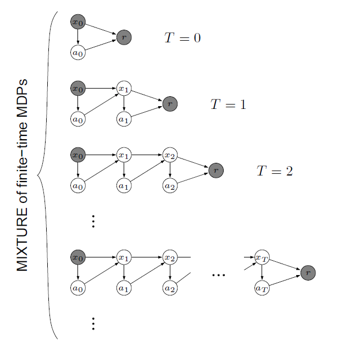
\includegraphics[width=0.6\linewidth]{mixMDP}
        \caption{Mixture of finite-time MDPs. Note this report uses notation that each finite-time MDP ends at time
                 $\Tau$ instead of $T$. Image courtesy of \cite{toussaint2010expectation}.}
        \label{fig:mixMDP}
    \end{figure}

    Their derivation starts with the joint distribution of the probability of a reward $\mathcal{R}$, a sequence of
    states $\traj$, and the probability of the sequence ending at time \Tau, subject to a policy $\policy{1}$. Note that
    $s^{(\Tau)}$ is the state at time $\Tau$ in the joint distribution,
    \begin{equation} \label{eq:em_joint_dist}
        \begin{split}
            P(R,\traj,\Tau;\policy{1})
                & = P(R|\traj;\policy{1})P(\traj|\Tau;\policy{1})P(\Tau) \\
                & = P(R|s^{(\Tau)};\policy{1})\left[\prod_{t=0}^{\Tau-1}P(s^{(t+1)}|s^{(t)};\policy{1})\right]
                        P(s^{(0)};\policy{1})\delta_{|\tau|\Tau}P(\Tau),
        \end{split}
    \end{equation}
    where $\delta_{|\tau|\Tau}=1$ when the trajectory ends at step $\Tau$ and is zero otherwise. The algorithm requires
    that each MDP in the mixture only emits a reward at a single final time step; the final states, $r$, in Fig.
    \ref{fig:mixMDP} emit rewards from the distribution $\mathcal{R}(s^{(\Tau)},a_1^{(\Tau)})$ which is defined:
    \[
    P(\mathcal{R}|s,a_t) = \frac{R(a_1,s) - \min_{a_1,s}(R)}{\max_{a_1,s}(R) - \min_{a_1,s}(R)}.
    \]

    \par
    The goal of EM is to maximize the following energy function,
    \[
    F(\policy{1},\omega) := \log P(\mathcal{R};\policy{1}) - KL(\omega(\tau,\Tau)||P(\tau,\Tau|\mathcal{R};\policy{1}).
    \]
    $F(\policy{1},\omega)$ is the difference between the log-likelihood of the reward probability subject to \policy{1},
    and the \ac{KLD} of the latent variable distribution $\omega$ from the latent variables given a reward and subject
    to $\policy{1}$. The latent, unknown, variables of the \ac{MDP} are the state-action sequence that brings the system
    to a final state, $s^{(\Tau)}$, at time $\Tau$. Note that only sequences where $|\traj|= \Tau$ provide a non-zero
    probability of reward in the mixture of finite-time \acp{MDP}.

    \par
    The M-step returns the energy function maximized over the latent variables using the previous, \textit{old},
    iteration's policy:
    \begin{equation} \label{eq:M_step}
        \begin{split}
            F(\policy{1},\omega^*)
                & = \sum_s \left[ P(\mathcal{R}|s^{(T)};\policy{1}^{old})\alpha(s)\right]
                        \log P(\mathcal{R}|s^{(T)};\policy{1}^{old}) \\
                &\quad\ \ + \sum_{s',s}\left[ \beta(s')P(s'|s;\policy{1}^{old})\alpha(s)\right]
                        \log P(s^{(t+1)}|s^{(t)};\policy{1}^{old}),
        \end{split}
    \end{equation}
    where
    \begin{align*}
        \alpha(s^{(t)}) & = \sum_{t=0}^\infty P(s^{(t)}; \policy{1}^{old})P(\Tau=t) \text{, and}\\
        \beta(s^{(t+1)}) & = \frac{1}{1-\gamma} \sum_{\upsilon=0}^{\infty}
            P(R|s^{(t)\prime},\Tau=t+\upsilon;\policy{1}^{old})P(\Tau=\upsilon+1).
    \end{align*}
    \noindent
    In the equation for $\beta$, above, the term $s^{(t)\prime}$ refers to reachable states from $s^{(t)}$.

    Essentially, the M-step provides a policy update. The E-step, given a policy, finds the state-action sequence that
    maximizes the expectation of a reward; the E-step calculates $\alpha$ and $\beta$. These two terms are then used in
    the M-step to provide the policy for future iterations, up to $Z$ iterations. The terms $\alpha$ and $\beta$ are
    updated on a state-action horizon time-limit of $H$.  Toussaint et al. in \cite{toussaint2010expectation} show that
    as $Z\rightarrow{}\infty$, and $H\rightarrow{}\infty$, the EM algorithm returns a policy equivalent to that from VI.
    The parameters $Z$ and $H$ are now added to the set of hyper-parameters for a multi-agent simulation

\begin{remark}
    In the experiment implementation in the following sections and chapters, note that if the horizon parameter $H$ is
    too short and the reward space is sparse, states that are too far from receiving a reward will select the
    \emph{Empty} action.
\end{remark}

    Section \ref{sec:em_vi_comparison} will compare the policy synthesis ov \ac{EM} and VI, but we first must define the
    true policy of \agent{2} in a multi-agent environment.




\section{Multi-agent Policy Model}\label{sec:multi_agent_model}

    When \agent{1} exists in the environment with \agent{2}, the state space in our \ac{HiPMDP}, $\mathcal{M}$, is again
    $S \equiv S_1 \times S_2$. In the case of the experiment in Section \ref{sec:single_agent_experiment}, the
    cardinality of $S$, $|S|$, has exploded to $25^2$. Given the number of actions available at each state, $5$, an
    approximation of $\policy{2}$ must represent the probability of selecting each action at each state; the cardinality
    of the policy estimate, $|\estimate{\policy{}}_2|$, has increased from $125$ to $3125$. How can we design a set of
    kernels, so that $K \ll |S|$ and minimize $\OneNorm{\policy{2}(s), \estimate{\policy{}}_2(s;\estimate{\paramVec})}$?


    For the example tasks described in Chapter \ref{chapt:motivation}, a human would infer that the uncontrollable
    agents would only change their actions if the controllable agent is within a relative distance. Other cars might
    only swerve away from a driver if two cars become dangerously close. Alternatively, a human holding a basket might
    only extend their arms to accept a load of items when the manipulator is sufficiently close to them. With this
    assumption, we'll make the inference task computationally manageable.

    For simplicity, we've adjusted the grid-world example from that used in Section \ref{sec:single_agent_experiment}
    one with no obstacles and deterministic transitions. The motivation for this will be discussed in Chapter
    \ref{chapt:proactive_inference}, but by limiting the stochasticity of the environment, the interactions of \agent{1}
    and \agent{2} are easier to influence.

\subsection{Fixed and Mobile kernels for policy inference}\label{sec:fixed_and_mobile_kernels}

\begin{assumption}\label{assump:multi_agent_interraction}
        The uncontrollable agent, \agent{2}, has a nominal policy, and when the agents are within some unknown distance
        $\mathsf{x}$, \policy{2} is biased either towards or away from the position of \agent{1}:
        \begin{align*}
        \policy{2} & = \begin{cases}
        f(s_2) & \text{if}\ \textnormal{SP}(s_1,s_2) > \mathsf{x} \\
        f(s_1,s_2) & \text{if}\ \textnormal{SP}(s_1,s_2) \leq \mathsf{x}.
        \end{cases} \\
        \end{align*}
\end{assumption}

    Using Assumption \ref{assump:multi_agent_interraction}, then we can segment our parameter and feature vectors into
    fixed and mobile elements. The fixed kernels are still scattered at locations $c_l \subset S_2,\ l=0,\ldots,K-1$.
    Now, consider that the next, $K^{\text{th}}$, kernel is mobile; it is attached to the \agent{1}\!'s location. When
    this kernel is far from the current state of \agent{2} its anticipated influence is very small due to Eq.
    \ref{eq:kernel_func}. This simply requires that another $|A|$ parameters elements are included in the \paramVec\
    from the experiments in Section \ref{sec:single_agent_experiment}.


\subsection{True Multi-Agent Policy of Agent 2} \label{sec:true_agent_2_multi_agent_policy}

    \begin{figure}[htb]
        \begin{center}
                \fbox{
                        \begin{minipage}{0.65\textwidth}
                            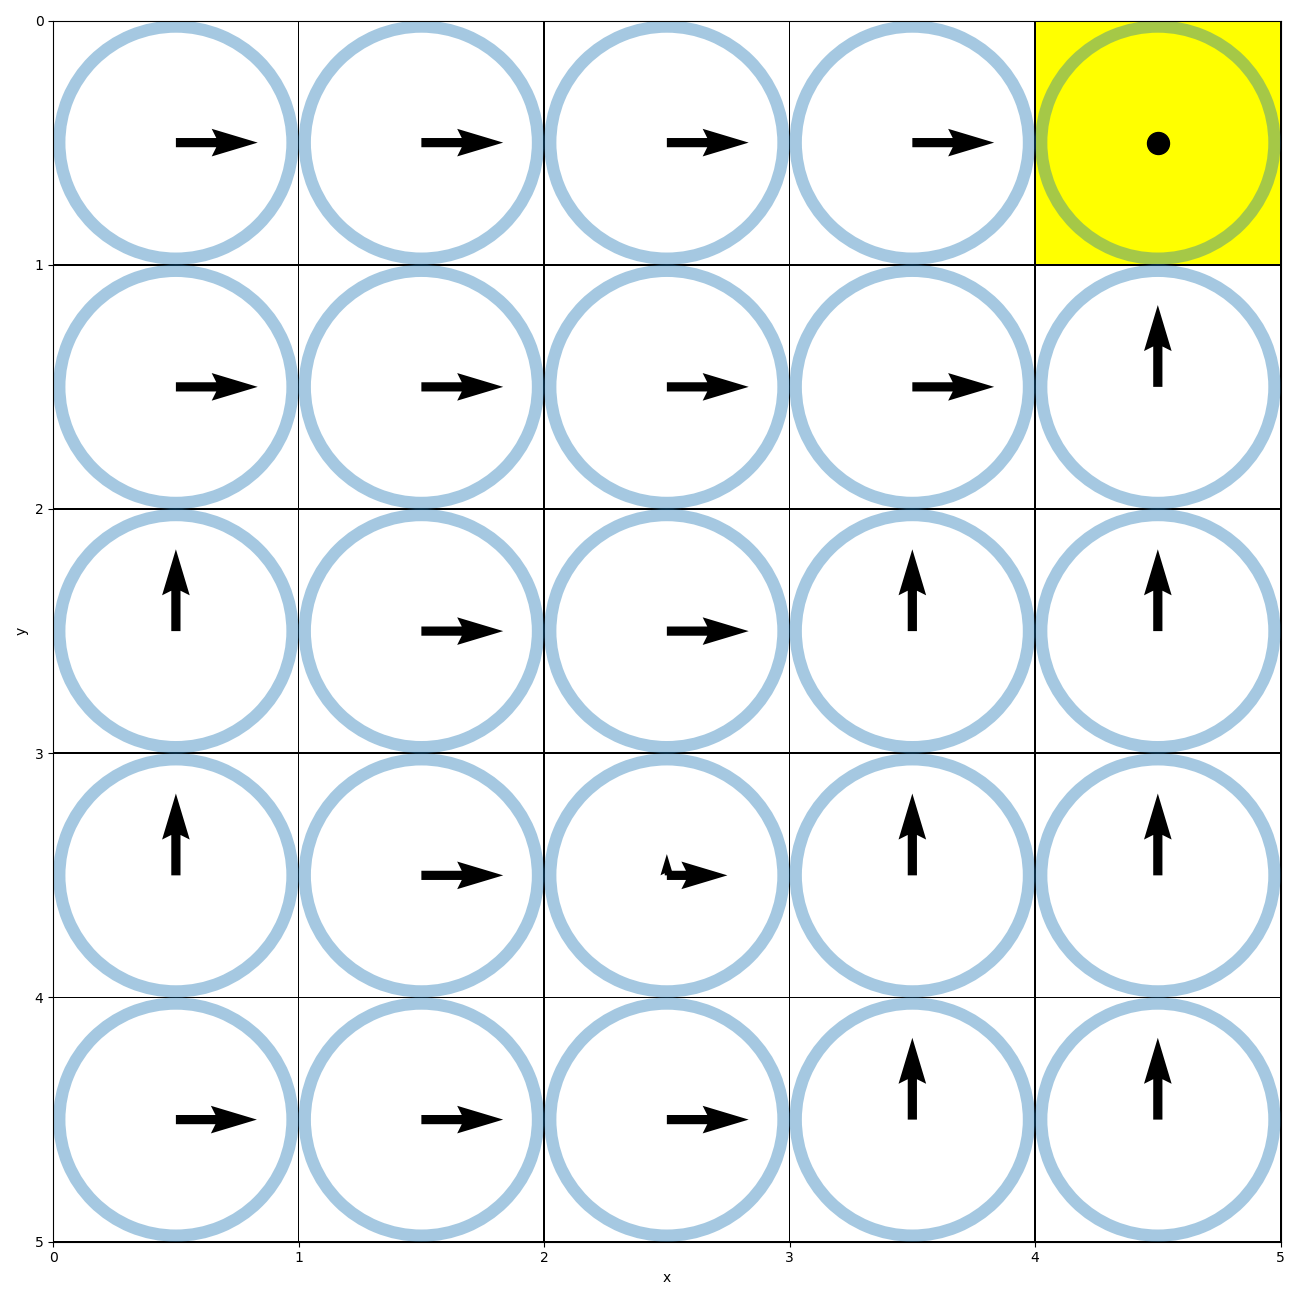
\includegraphics[width=\textwidth]{single_agent_empty_learned}
                            \caption{Hidden Policy of \agent{2} in an empty, deterministic, world.}
                            \label{fig:single_agent_empty_policy}
                        \end{minipage}
                }
        \end{center}
    \end{figure}

    To perform multi-agent experiments, let's now synthesize a true policy for \agent{2} that is a combination of the
    policy shown in Fig. \ref{fig:single_agent_empty_policy} and a repulsive effect from the proximity to \agent{1}. To
    form the policy in Fig. \ref{fig:single_agent_empty_policy}, the experiment in Sec.
    \ref{sec:single_agent_25K_results} was repeated, thus the light-blue kernel markers on each grid-cell. With these
    inference results, we have a set of parameters, $\optimal{\paramVec}_{\mathsf{FIXED}}$ that satisfy Assumption
    \ref{assump:opt_policy_err} for that stationary distribution such that the true \emph{Q}-function of \agent{2} is:
    \[
        Q(s,a_2) = \estimate{Q}(s,a_2; \optimal{\paramVec}_{\mathsf{FIXED}})
                 = \sum_{\paramIdx=1}^{\paramLen_{\mathsf{FIXED}}} \optimal{\paramSym}_{\paramIdx} \featElem(s,a_2),
    \]
    where $W_{\mathsf{FIXED}}=K_{\mathsf{FIXED}}\times |A|$ and $K_{\mathsf{FIXED}}=25$ and $|A|=5$. These 25 kernels
    are at fixed locations in the grid-world.

    To represent the repulsion that \agent{2} should desire as it \agent{1} approaches, we'll attach a single mobile
    kernel to the location of \agent{1}. The kernel function for this kernel is identical to Eq. \ref{eq:kernel_func},
    except that its center is mobile: $c_{\mathsf{MOBILE}} = s_1^{(t)}$ for all $t \in [0,|\traj|)$. With the associated
    feature-function $\phi_{\mathsf{MOBILE}}$, we'll associate five parameter values that will decrease the value of
    \agent{2}'s \emph{Q}-function if \agent{1} is close. All the parameters used to synthesize a true policy for
    $\agent{2}$ are:

\begin{table}[H]
    \centering
    \begin{tabular}{l|l l}
        $\optimal{\paramVec}_{\mathsf{FIXED}}$ & -- & Results used for Fig. \ref{fig:single_agent_L1Norm_25_kernels} \\
        $c_{\mathsf{FIXED}}$ & -- & Grid Cells $0,\ldots 24$ \\
        $\sigma_{\mathsf{FIXED}}$ & $2.0$ & Fixed kernel standard deviations\\
        $c_{\mathsf{MOBILE}}$ & -- & Described above \\
        $\kernStdDev_{\mathsf{MOBILE}}$ & $\mathbf{1.0}$ & Mobile kernel standard-deviations.\\
        $\theta_{\mathsf{MOBILE}\ \forall\ a \in\ \{N,S,E,W\}}$ & $-0.9$  & Negative action value for ${North, South,
                                                                                                        East, West}$\\
        $\theta_{\mathsf{MOBILE}\ a = \{Empty\}}$ & $0.0$  & No additional weight for $Empty$ action \\
        $\kappa$ & $1.0$ & Temperature of $\policy{2}(s)$ Eq.\ref{eq:policy_model} \\
    \end{tabular}
    \caption{Parameters to synthesize hidden $\policy{2}((s_1,s_2))$.}
    \label{table:true_multi_agent_2_policy}
\end{table}

    The resulting policy is harder to visualize. In Figure \ref{fig:agent_2_multi_agent_policy}, the black arrow
    magnitudes represent the probability of \agent{2} taking each action \textbf{given that \agent{1} is located in the
    blue cell}. Grey dots become larger and blacker as the probability of \agent{2} selecting the \emph{Empty} action
    increases. The effect of the mobile kernel is obvious in comparison to Figure.  \ref{fig:single_agent_empty_policy}.
    This realization of $\policy{2}((s_1,s_2);\optimal{\paramVec})$ will be used as the benchmark for multi-agent
    inference experiments in both Section \ref{sec:multi_agent_inference_experiment} and Chapter
    \ref{chapt:proactive_inference}.

    \begin{figure}[htb]
        \begin{center}
                \fbox{
                        \begin{minipage}{0.65\textwidth}
                                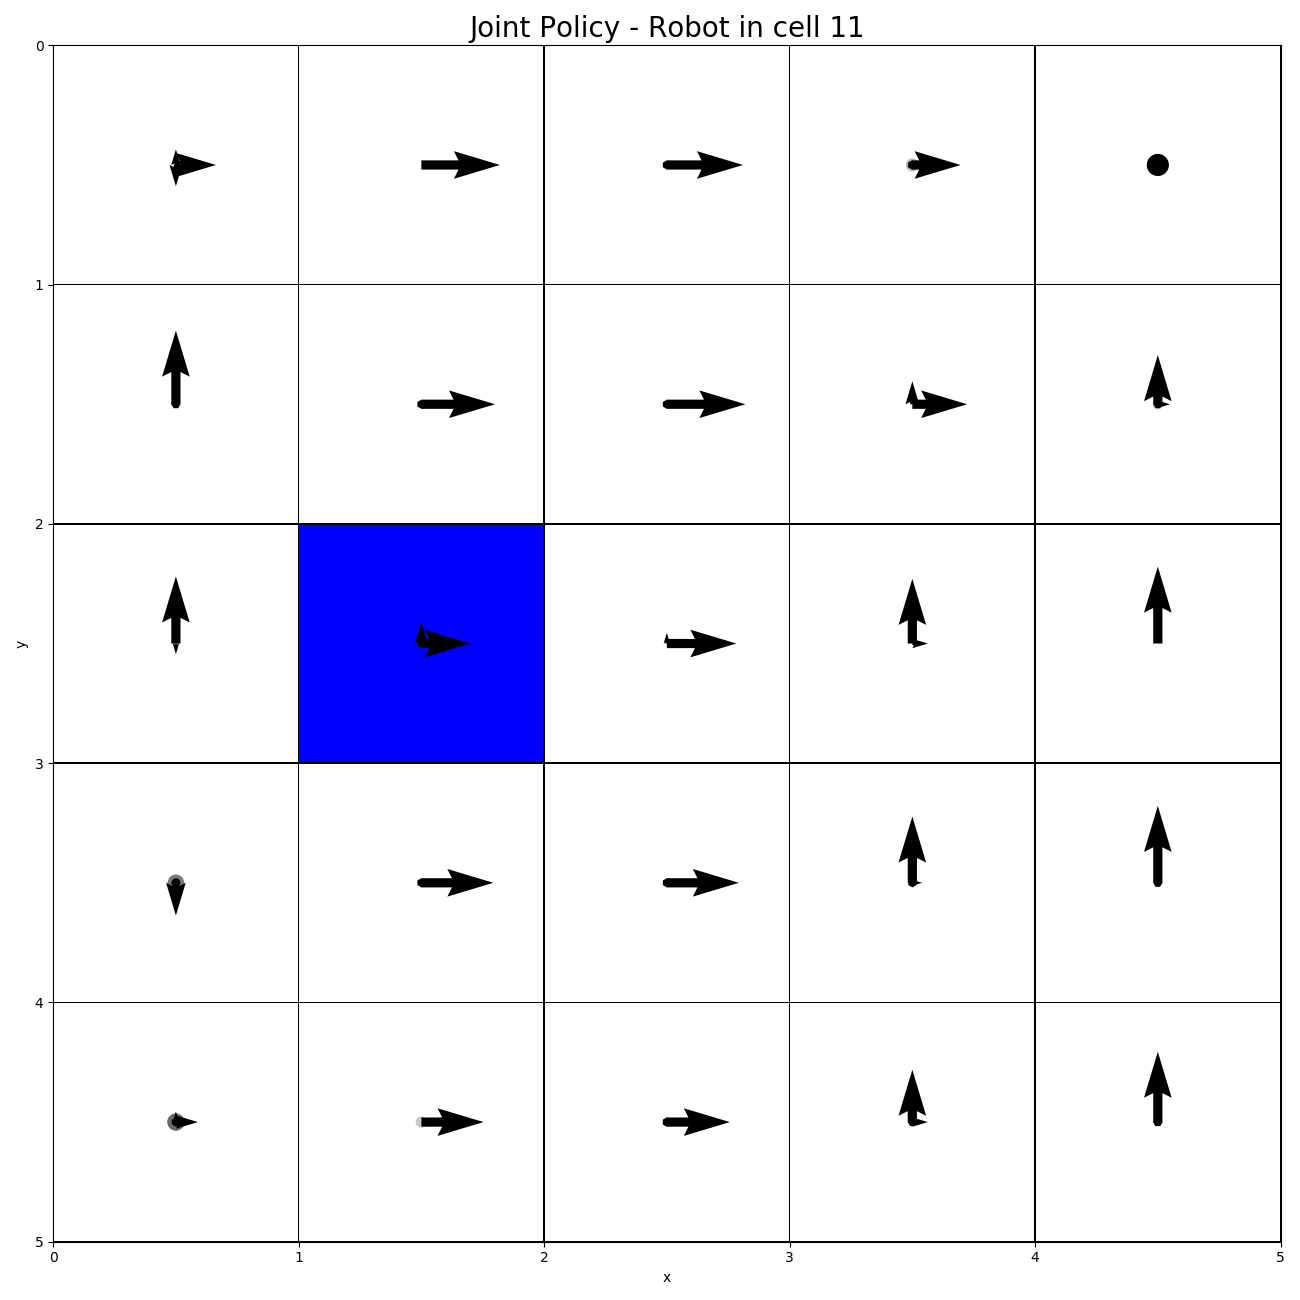
\includegraphics[width=\textwidth]{agent_2_multi_agent_policy}
                                \caption{Hidden Policy of \agent{2} in an empty, deterministic, world with $s_1=11$.}
                                \label{fig:agent_2_multi_agent_policy}
                        \end{minipage}
                }
        \end{center}
\end{figure}


\section{Policy Synthesis Comparison} \label{sec:em_vi_comparison}
In future experiments, \agent{1} will be tasked to reach the upper left (\emph{North-West} grid cell, $s_1=0$,
\emph{without} landing in the same cell as \agent{2}. The reward function for \agent{1} is
\begin{align*}
        R(s,a_1) & = \begin{cases}
1 & \text{if}\ s_1 == 0, \forall s_2 \in S_2\ \&\ a_1==Empty \\
0 & \text{Otherwise} \\
\end{cases} \\
\end{align*}
In the case that $s_1==s_2$, the transition probability of $\mathcal{M}$ is set to a self-loop under all actions.

To create a bencmark optimal policy for \agent{1}, $\policy{1}(s;\optimal{\paramVec})$, we'll solve Eq.
\ref{eq:bellman_true} with \ac{VI} and maximize Eq. \ref{eq:M_step} using $\policy{2}((s_1,s_2);\optimal{\paramVec})$.
The parameters necessary for EM and VI are listed in Table \ref{table:optimal_agent_1_EM_policy_params}.

\begin{table}[htb]
        \centering
        \begin{tabular}{l|l l}
                $\gamma$ & $0.9$ & Discount rate in $\mathcal{M}$ \\
                $Z$ & 100 & EM-only: Number of M-step evaluations \\
                $H$ & 15 & EM-only: Trajectory Horizon Length \\
        \end{tabular}
        \caption{Parameters to synthesize optimal $\policy{1}((s_1,s_2);\optimal{\paramVec})$.}
        \label{table:optimal_agent_1_EM_policy_params}
\end{table}
As a comparison, when \emph{agent two} is in the middle cell, marked in blue, the optimal policy of \agent{1} to reach
the green cell is shown in Figure \ref{fig:optimal_agent_1_VI_policy}. The agent is clearly exploiting its knowledge of
the true $\policy{2}(s;\optimal{\paramVec})$ when $(s) = (13,12)$ as that is normally a very dangerous
action\footnote{Actually, a bug was recently discovered in the simulation engine written by your's truly. Without a
memory variable in the MDP, the agent's are currently allowed to \emph{swap} places without triggering a collision. The
root of the problem is the definition of the transition probability matrix format and is not an easy fix. However, the
policy of \agent{1} cleraly exploits this when $(s) = (13,12)$ (the blue cell is 12, the one to the right of it is cell
13).}. Figure \ref{fig:optimal_agent_1_EM_policy} shows the approximately optimal $\policy{2}(s;\optimal{\paramVec})$
from EM.

    \begin{figure}[htb]
        \begin{center}
                \fbox{
                        \begin{minipage}{0.65\textwidth}
                                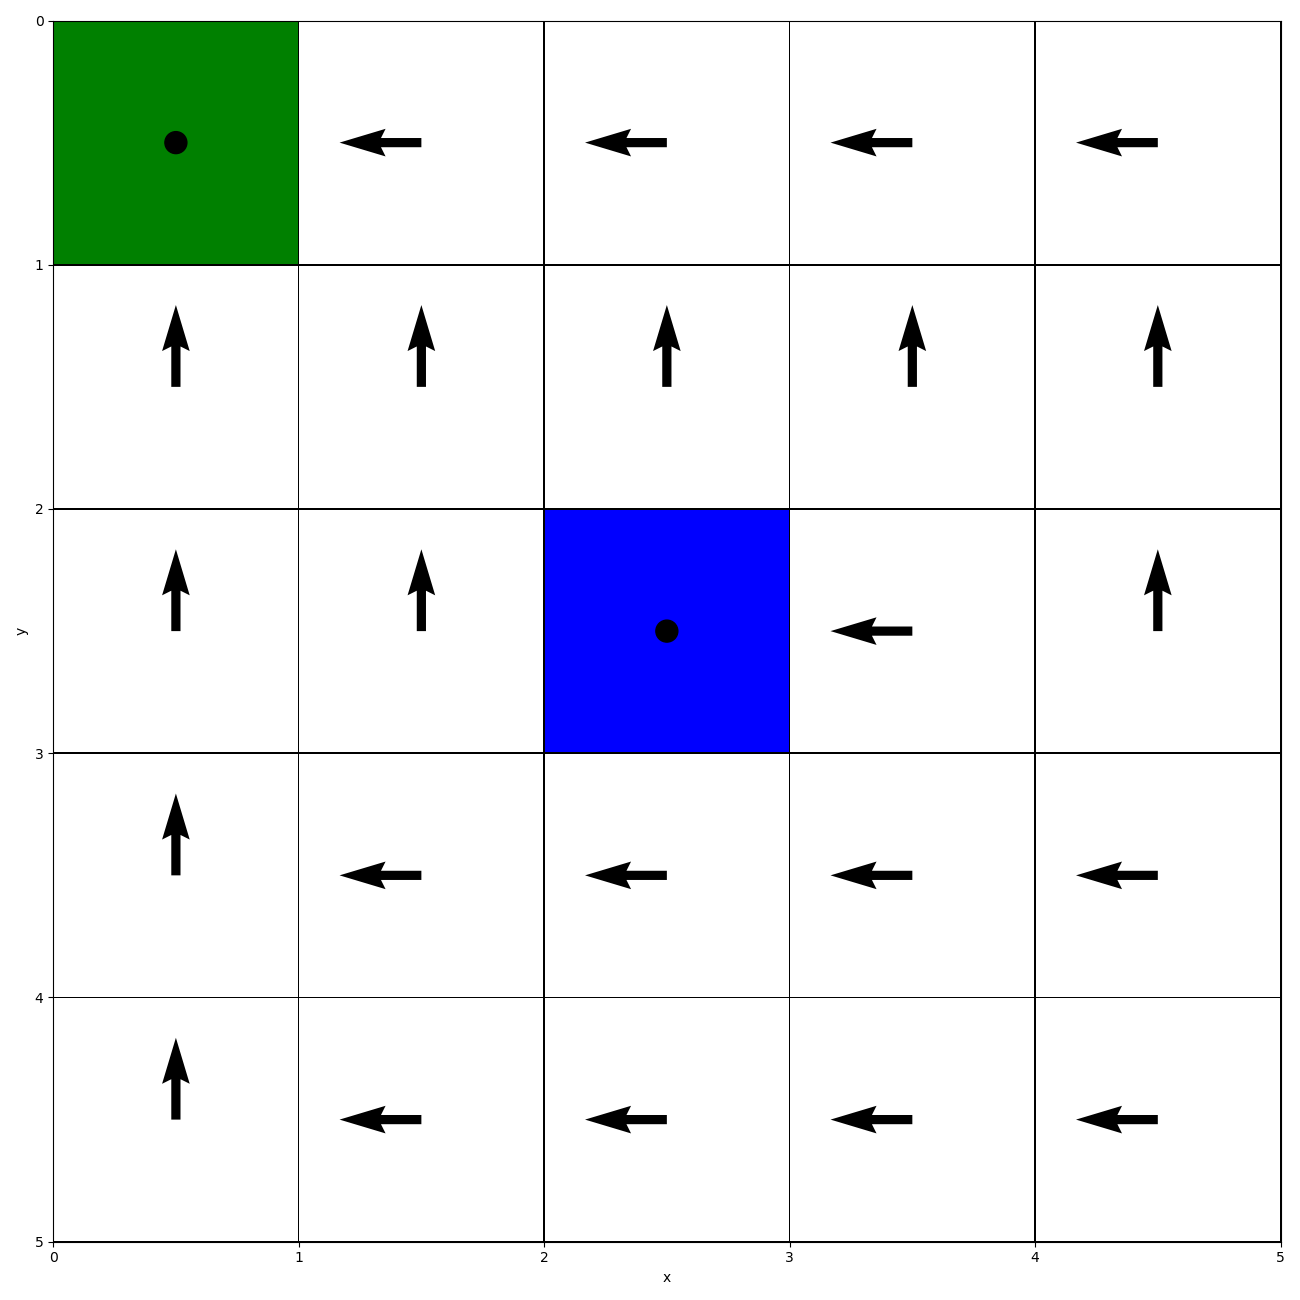
\includegraphics[width=\textwidth]{optimal_robot_VI_policy}
                                \caption{Optimal policy of \agent{1} from VI with $s_2=12$.}
                                \label{fig:optimal_agent_1_VI_policy}
                        \end{minipage}
                }
        \end{center}
\end{figure}

    \begin{figure}[htb]
        \begin{center}
                \fbox{
                        \begin{minipage}{0.65\textwidth}
                                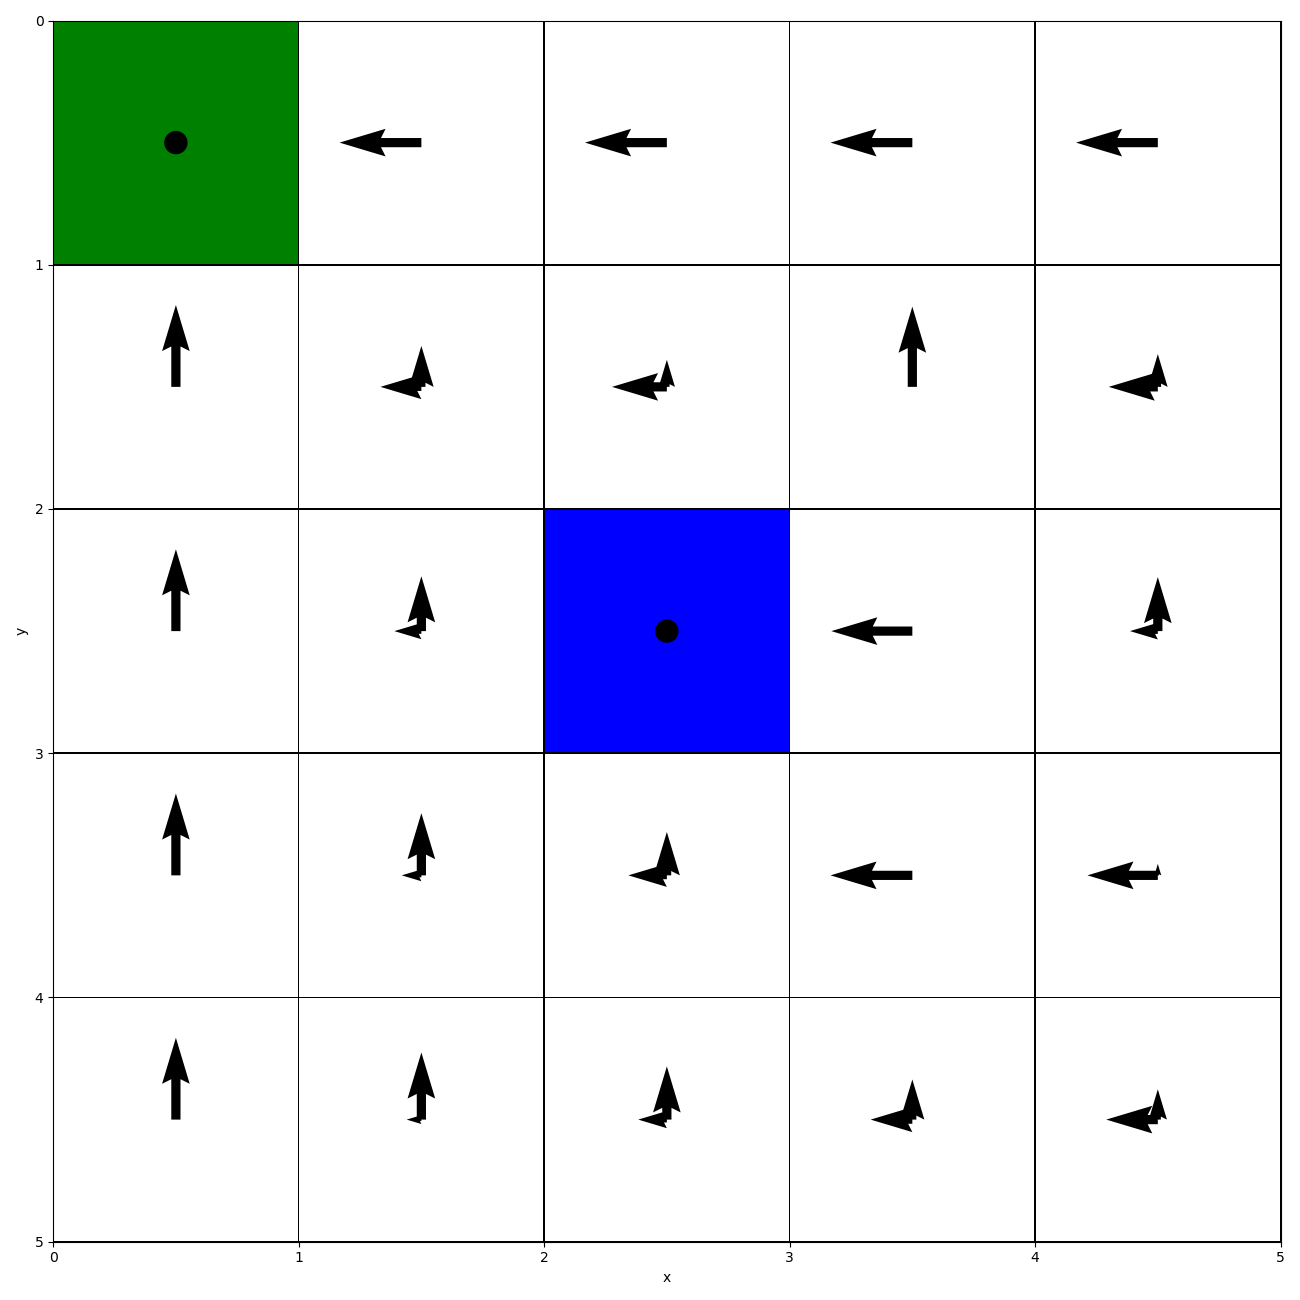
\includegraphics[width=\textwidth]{optimal_robot_EM_policy}
                                \caption{Approximately optimal policy of \agent{1} from EM with $s_2=12$.}
                                \label{fig:optimal_agent_1_EM_policy}
                        \end{minipage}
                }
        \end{center}
\end{figure}

\section{Multi Agent Inference Experiment}\label{sec:multi_agent_inference_experiment}
Using the observed data-set described by Table \ref{table:multi_agent_data_set} we can perform similar experiments to
those in Section \ref{sec:single_agent_experiment}. We'll also use the inference parameters in Table
\ref{table:multi_agent_hyper_params} that notes, among other things, that this experiment uses $25$ fixed kernel
locations and a mobile kernel.

The error metric plotted in Fig. \ref{fig:multi_agent_error_25_kernels} is now the fraction of the maximum possible
$\text{L}_1$-norm. That is, for each iteration $n$,
\begin{equation}\label{eq:error_percent}
        Error(n) = \frac{\OneNorm{\policy{2},\estimate{\policy{}}_2}}{2|S|}.
\end{equation}
With this, we can represent the likelihood of $\estimate{\policy{}}_2$ selecting different actions at each joint state
$s$ from the true \policy{2}. For instance, if $Error(n)==1$, then all actions sampled from $\estimate{\policy{}}_2$
will be different from the true \policy{2} at every state. Recognize that there are infinitely many softmax policies
that have $Error(n)==1$, and a finite number of hardmax policies with this upper error value.

Given that the feature-space is much smaller than the joint state-action-space, $W = 26 \times 5 = K \times |A| \ll
|S|\times |A| = 625 \times 5$, the inference result in Fig. \ref{fig:multi_agent_error_25_kernels} produced a reasonable
policy estimate, $\estimate{\policy{}}_2$.


\begin{table}[H]
        \centering
        \begin{tabular}{c|l l}
                $|\traj|$ & $10$ & Number of steps in a trajectory \\
                $|D|$ & $3000$ & Number of trajectories observed \\
                $I_0$ & $\big(\mathcal{U}(0,24), \mathcal{U}(0,24)\big)$ & Uniform distribution of $s^{(0)}$ \\
        \end{tabular}
        \caption{Observed data for multi agent inference.}
        \label{table:multi_agent_data_set}
\end{table}

\begin{table}[H]
        \centering
        \begin{tabular}{c|l l}
                $\kernStdDev_{\kernIdx}$ & $2.0,\ \forall l$ & Identical kernel standard-deviations for all mobile and
                                                               fixed kernels\\
                $c_{\kernIdx}$ & -- & (Kernel Centers) Grid Cells $0,\ldots 24 \cup s_1^{(t)}$\\
                $\kappa$ & $0.5$ & Temperature of $\estimate{\policy{}}_2$. Eq. (\ref{eq:policy_model}) \\
                $\lambda$ & $1\mathrm{e}\!-\!5$ & Gradient update rate. Eq. (\ref{eq:gradient_update}) \\
                $\eta$ & $0.0$ & Gradient velocity memory\\
                $m$ & 2000 & Per iteration sample size of $\paramVec\sim \rho$\\
                $\Lambda$ & $60$ & Moving average buffer length for $\mathsf{HIST}(\logLike)$ \\
                $\zeta$ & $0.001$ & Gradient ascent termination when $\Delta\mathsf{HIST}(\logLike) < \zeta$\\
                $\mu_{0}$ & $0.0$ & Initial parameter means\\
                $\nu_{0}$ & $1.0$ & Initial parameter standard-deviations\\
                $\nu_{min}$ & $0.2$ & Minimum parameter standard-deviation\\
        \end{tabular}
        \caption{Hyper-parameters used for multi-agent inference.}
        \label{table:multi_agent_hyper_params}
\end{table}

    \begin{figure}[htb]
        \begin{center}
            \fbox{
                \begin{minipage}{0.75\textwidth}
                    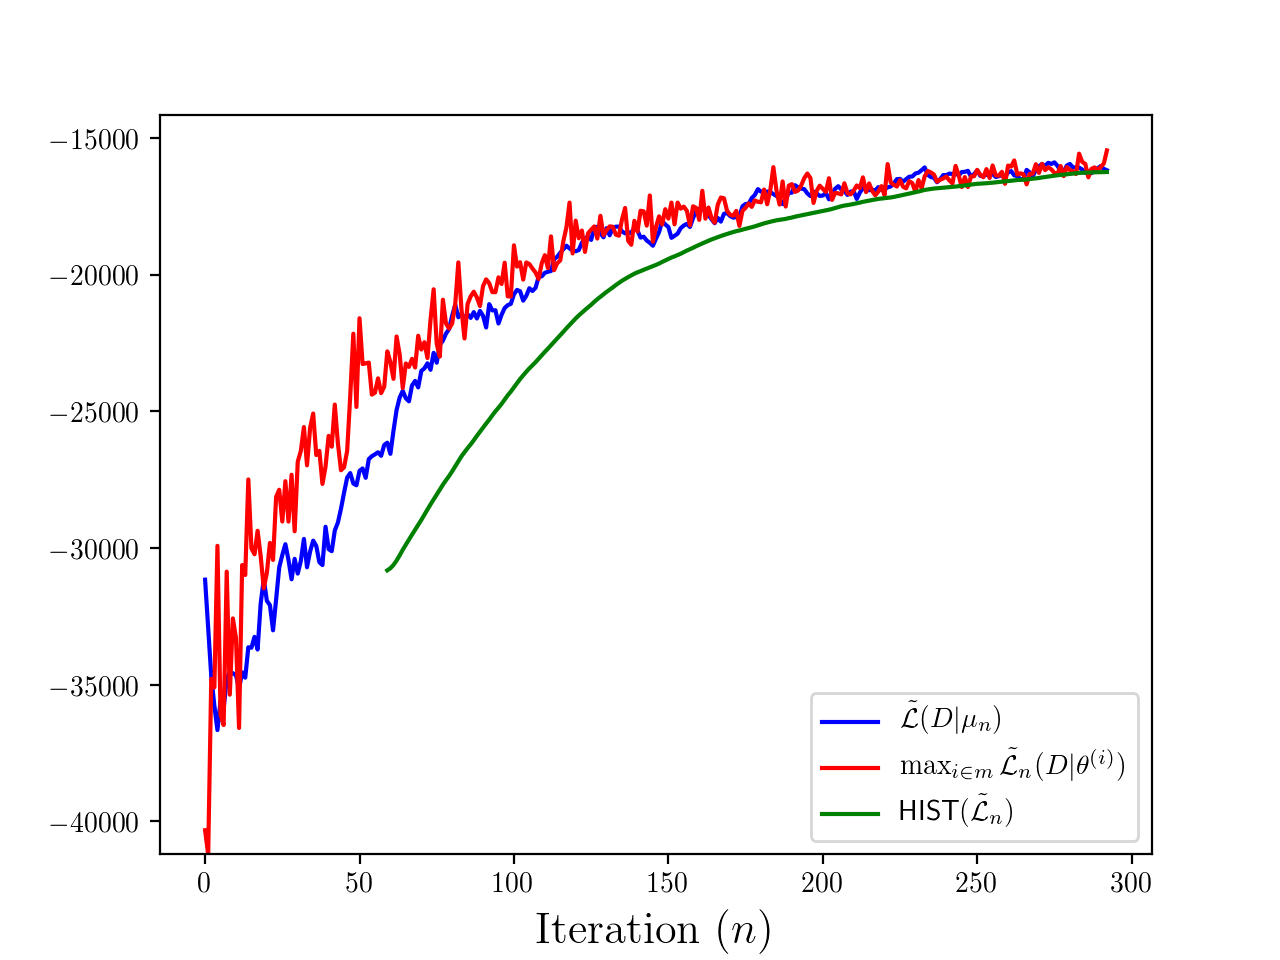
\includegraphics[width=\textwidth]{loglike_multi_agent_25K}
                    \caption{$\tilde{\logLike}(D|\rho)$ with parameters in Table \ref{table:multi_agent_hyper_params}.}
                    \label{fig:multi_agent_logLike_25_kernels}
                \end{minipage}
            }
        \end{center}
\end{figure}


\begin{figure}[htb]
        \begin{center}
                \fbox{
                    \begin{minipage}{0.75\textwidth}
                        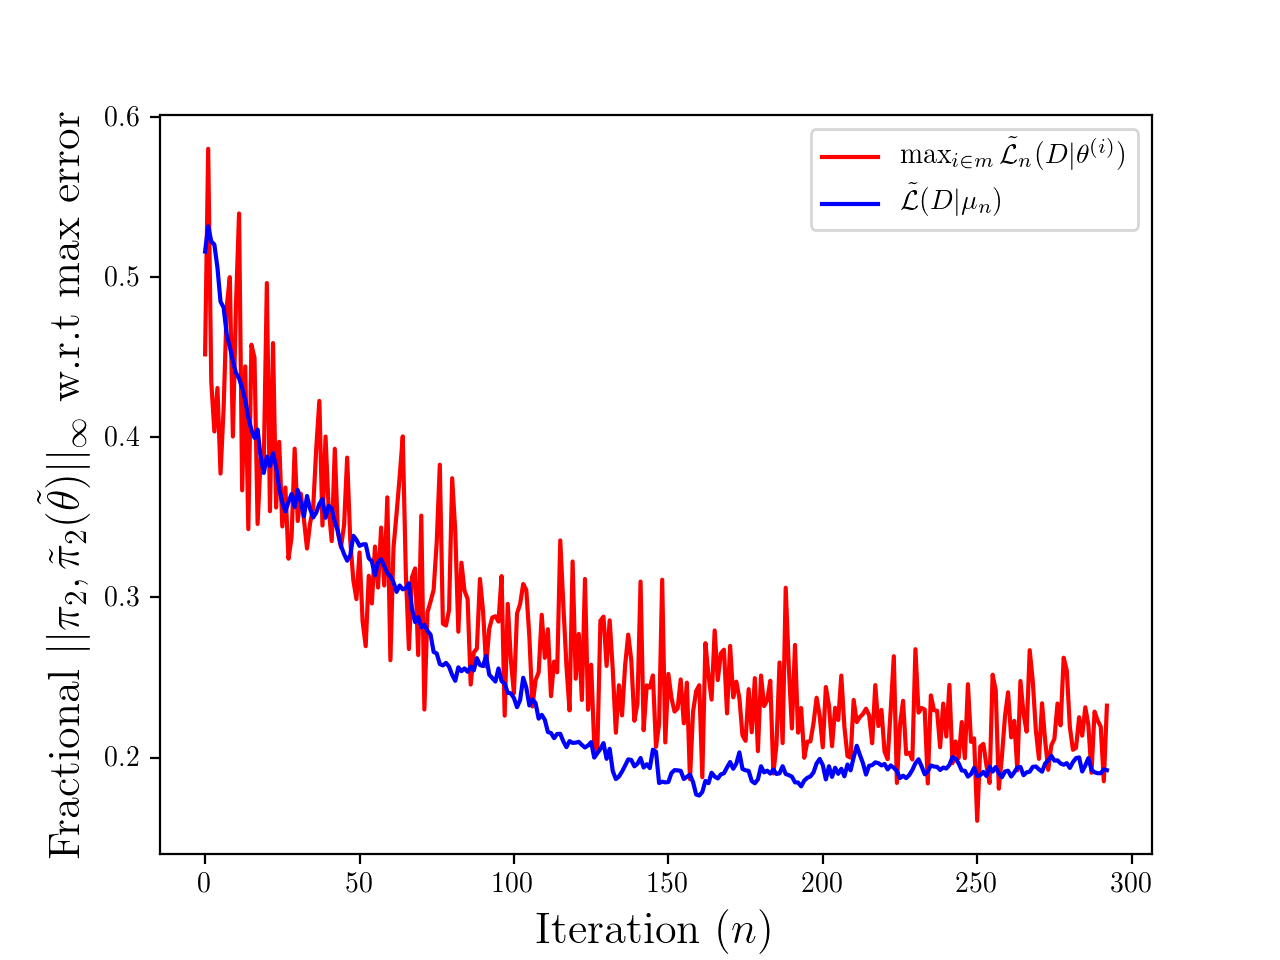
\includegraphics[width=\textwidth]{error_multi_agent_25K}
                        \caption{Fraction of max $\OneNorm{\policy{2},\estimate{\policy{}}_2}$ with parameters in Table
                                \ref{table:multi_agent_hyper_params}.}
                        \label{fig:multi_agent_error_25_kernels}
                    \end{minipage}
	                }
        \end{center}
\end{figure}

        \begin{figure}[htb]
        \begin{center}
            \fbox{
                \begin{minipage}{0.75\textwidth}
                    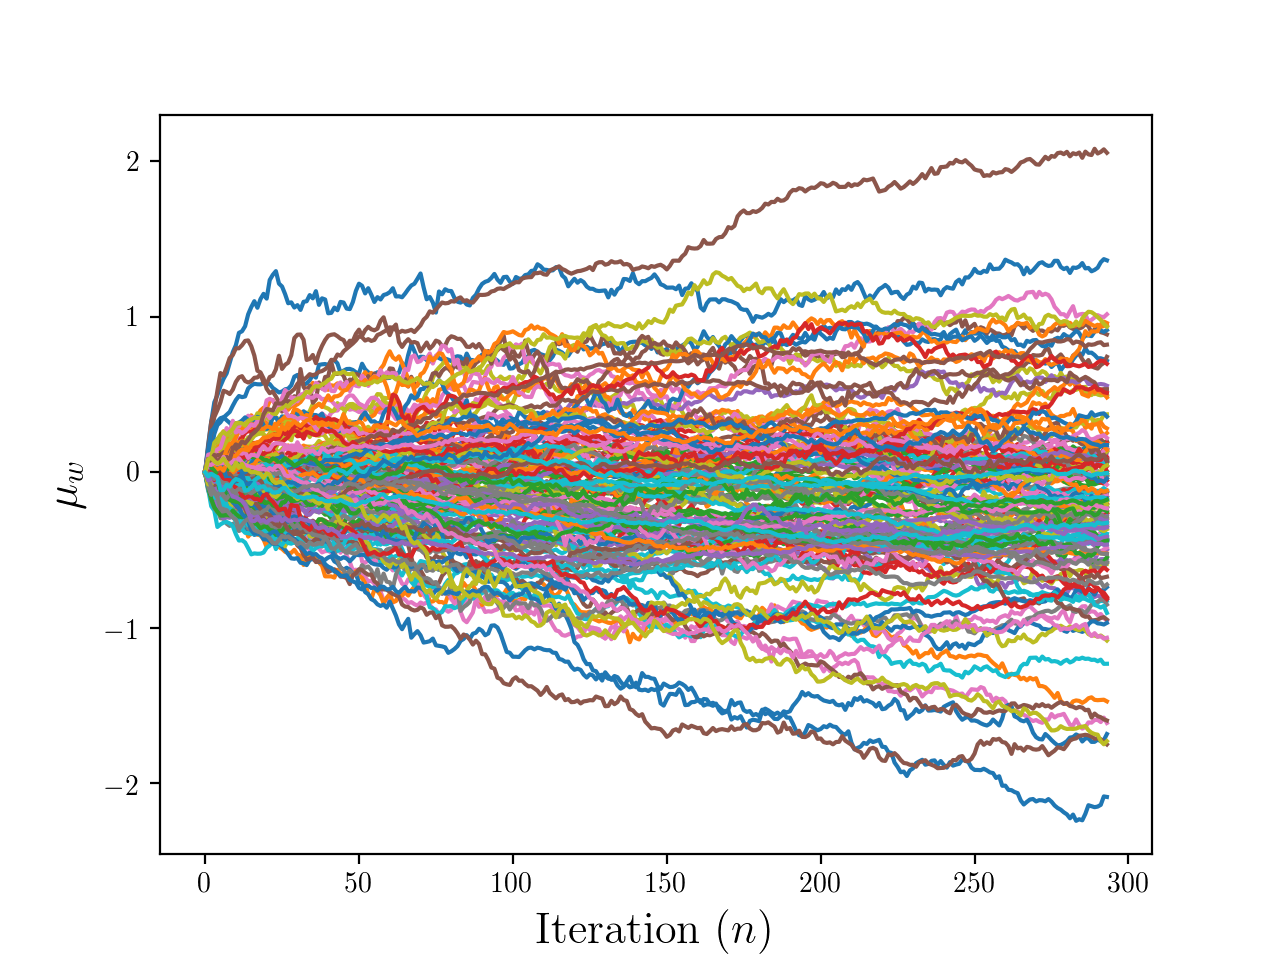
\includegraphics[width=\textwidth]{multi_agent_25K_mu}
                    \caption{$\mu_w$ for each iteration with parameters in Table
                    \ref{table:multi_agent_hyper_params}.}
                    \label{fig:multi_agent_25K_mu}
                \end{minipage}
            }
        \end{center}
\end{figure}

\begin{figure}[htb]
        \begin{center}
                \fbox{
                        \begin{minipage}{0.75\textwidth}
                                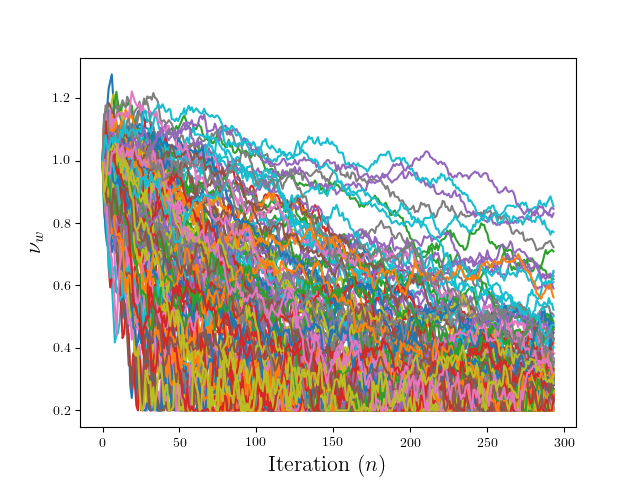
\includegraphics[width=\textwidth]{multi_agent_25K_nu}
                                \caption{$\nu_w$ for each iteration with parameters in Table
                                \ref{table:multi_agent_hyper_params}.}
                                \label{fig:multi_agent_25K_nu}
                        \end{minipage}
                }
        \end{center}
\end{figure}
